\documentclass[11pt]{article}

\author{Evan Dreher}
\date{March 2026}
\title{Science of Cybersecurity Attack Project: The Man in the Middle}

\usepackage{graphicx}
\usepackage{amsthm,amssymb,amsfonts,amsmath}

\begin{document}
\maketitle

\section{Setup}

\subsection{The Network}
\par The premise of this project is that an attacker tries to sniff the packets of the victim who is communicating with some server. In order to do this, the first thing necessary is a server-client-attacker network. The host machine acted as the server. The attacker and client were virtual machines created on Oracle VM VirtualBox. Both VirtualBox machines were configured with a Host-only adapter so that the host machine and the virtual machines could communicate with each other over an isolated network where the attack would take place.

\par During the demonstration, the attacker poisons the ARP tables of the isolated network thus inserting themself between the server and client. The victim then accesses the web server and the attacker is able to view their data.

\subsection{Web Service}
\par Once the network was set up, the next thing necessary is a web application that the client can connect to and the attacker can spy on.  The app designed for this project is a small phony banking service written using Python's Flask framework. WTForms was used to handle user input and SQLAlchemy for database interactions. The app supports very basic banking functions such as user authentication, account creation, deposits, wire transfers, and account transaction history. User passwords are hashed with the Argon2 hasing algorithm before being stored in the database.

\subsection{The Attacker VM}
\par The attacker's VM is going to act as the ``Man-in-the-middle'' (MITM) in this attack. All of the coding done by the attacker is in the form of Linux terminal commands (AKA bash). For the sake of the demonstration these commands have been loaded into three bash scripts which are stored on the attacker's machine. They will use these scripts to spoof the IP addresses of the server and victim so that the attacker can view all their communications.

\section{Attack Scenarios}

\subsection{Stealing Credentials via MITM}
\subsubsection{Steps of the Attack}

\begin{enumerate}
    \item The attacker enables IP packet forwarding,
    \item finds the subnet mask of the network and finds all hosts connected to it via \texttt{arp-scan},
    \item spoofs the IP addresses of the server and client by sending false ARP replies via \texttt{arpspoof} (see figure \ref{fig:phase2}),
    \item and listens to all TCP communications they hear and dumps them into a \texttt{.pcap} file to be read later (see figure \ref{fig:tcpdump}).
    \item The victim logs in with their credentials and the packets get routed through the attacker's VM.
    \item The attacker scans through the \texttt{.pcap} file to find which routes the victim visited as well as observe the query parameters sent between them which includes their login credentials.
    \item The attacker is able to log in to the victim's account with their stolen credentials
\end{enumerate}

\begin{figure}[h!]
\begin{center}
    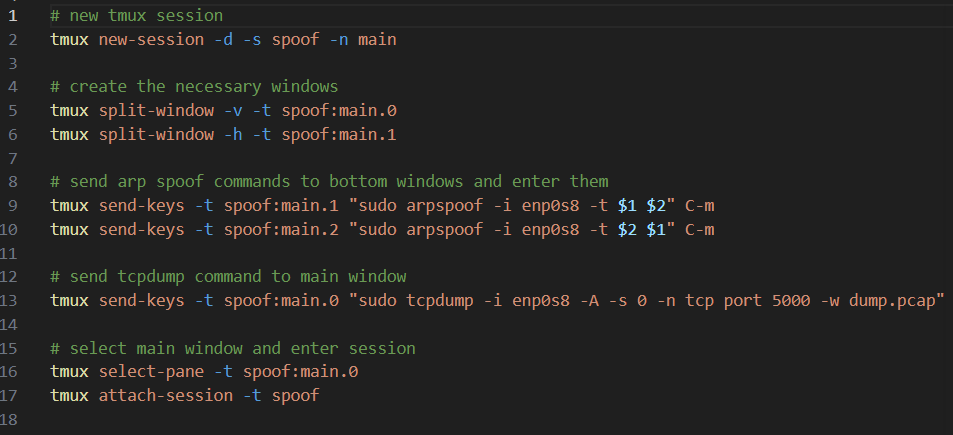
\includegraphics[width=4in]{figures/bash.png}
    \caption{Bash script taking 2 parameters used to poison the ARP tables of the LAN}
    \label{fig:phase2}
\end{center}
\end{figure}

\begin{figure}[h!]
\begin{center}
    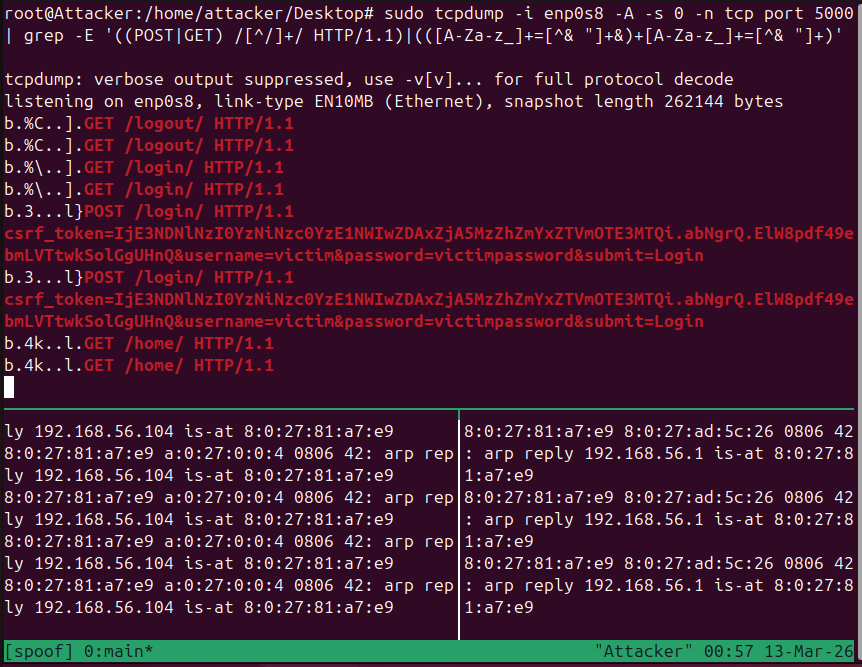
\includegraphics[width=4in]{figures/tcpdump.png}
    \caption{Attacker view of TCP traffic}
    \label{fig:tcpdump}
\end{center}
\end{figure}

\subsubsection{Vulnerability}
\par The attack relies on two vulnerabilities. The first is the lack of authentication in ARP, and the second is the unencrypted communication in HTTP.

\par Address Resolution Protocol is used on a local network to map IP addresses to MAC addresses. In order for a machine to communicate with others on the network, it broadcasts an ARP request asking for the MAC address of the machine that owns a particular IP address. The problem is, any device on the network can reply claiming to be the owner of the requested address. Furthermore the requesting machine trusts any reply it recieves for the request, updating its cached ARP table accordingly. Due to the lack of authentication, an attacker who knows the IP addresses of the server and victim can send out false ARP replies to redirect network traffic as they see fit (through their machine in this demonstration).

\par The second vulnerability is the use of HTTP rather than HTTPS for communication with the server. HTTP sends all data as plaintext so if it is intercepted at all there is no further defense against leaking the communicated data. In the demonstration for this project, this will include login credentials for the victim's bank account. Since the data is unencrypted, the MITM will be able to view it as plaintext and steal the information.

\subsubsection{Attack Surface}
\par The attack surface for this demonstration is the LAN connecting the client and server. Since its a shared network, the attacker can manipulate the network communications between client and server using standard protocols such as ARP and HTTP to directly observe and interact with the communications.

\subsubsection{Attack Vector}
\par The attack vector is the ARP spoofing (also known as ARP poisoning) used to interfere with the connection between client and server. The attacker broadcasts false ARP replies to the server and client, and since ARP does no authentication, both machines will be tricked into assocating the attacker's MAC address with the other machine's IP address.

\par The exploits for this project are the bash commands the attacker uses to insert themself between server and client and view the communications; namely \texttt{arp-scan}, \texttt{arpspoof}, and \texttt{tcpdump}. The use of these commands allows the attacker to reroute all traffic through their machine and see data being transferred in real time as seen in figure \ref{fig:tcpdump}. In the figure we see a linux terminal split three ways. The two bottom terminals are performing the ARP spoofing, with one terminal broadcasting messages to the network that the server's IP address is located at this MAC address and the other doing the same fore the client's IP address. In those terminals you see the message is printed several times, this is because the ARP spoofing sends out broadcasts every second to make sure the ARP tables stay updated with the attacker's MAC address. In the top terminal, we see the communications happening between the server and client, \texttt{grep} was used to filter the traffic so we only see the routes the victim visited as well as query parameters which include their login credentials ``username=victim'' and ``password=victimpassword.''

\subsubsection{Why the Attack Works}
\par The success of this attack is due to the complete lack of security in both protocols (ARP and HTTP). The design of these protocols in conjunction with one another allows an attacker to impersonate other devices so they can reroute traffic and view unencrypted data.

\par As stated previously, the ARP model requires no authentication and trusts all incoming replies; updating ARP caches accordingly. This makes it very easy for other hosts on the network to impersonate other machines and reroute traffic which is the core principle of the attack. However, even though the attacker can do this, their plan would still be foiled if it weren't for the fact that all communications are also unencrypted. It would be okay for the attack to sniff packets if all the packets were unreadable, but without TLS provided by HTTPS the attacker can easily expose sensitive data.

\subsection{Alternate Scenario - Modifying Incoming Requests}
\par As the MITM, the attacker can do more than just view incoming and outgoing communications between the client and server. With a tool like \texttt{mitmproxy}, they can actually stop an incoming request, modify it, and then pass it along. This allows them to impersonate the client without ever having to actually sign on to their account. For example, if the victim sent out a request to perform a wire transfer the attacker would see something like
\begin{align*}
    & \texttt{POST http://192.168.56.1:5000/transfer} \\
    & \texttt{from\_account=victim\_account} \\
    & \texttt{to\_account=other\_account} \\
    & \texttt{amount=100}\$
\end{align*}

\par They could then pause that request, change the field ``\texttt{to\_account}'' to their own account, and forward it along. The money would then be sent to the attacker, and until the person that the money was supposed to be sent to says something the victim may be none the wiser. By default, \texttt{mitmproxy} is a bash command, but it is also comes in the form of a python library which has the same functionality. With the python library its even possible to automate this process causing many transfers over the network to be rerouted without additional work from the attacker. This would also significantly shorten the time that the request is paused which will help keep the victims unaware.

\subsection{Alternate Scenario - Denial of Service}
\par The first step of this demonstration was for the attacker to enable packet forwarding. Packet forwarding is a kernel feature of the linux machine that the attacker is using. When enabled, the attacker's machine acts as a router; it recieves incoming packets, and then forwards them along to their destination. By default this feature is disabled, and if the attacker performs the exact same steps as the first scenario but with packet forwarding disabled, then all outgoing requests sent by the victim will be routed to the attacker and stop there. This makes it impossible for the client to connect to establish a connection with the server which results in errors like in figure \ref{fig:noconnect}.

\begin{figure}[h!]
\begin{center}
    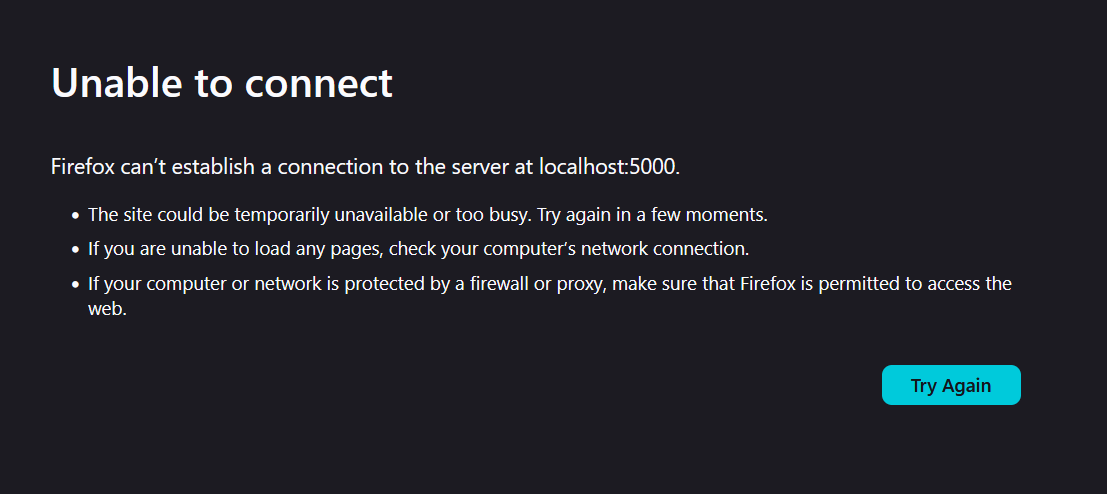
\includegraphics[width=4in]{figures/noconnect.png}
    \caption{Client fails to connect since Attacker isn't forwarding their packets}
    \label{fig:noconnect}
\end{center}
\end{figure}

\par This effectively cuts the client out of the network denying them services they would recieve from the internet.

\section{Conclusion}
\par The primary thing to note about this project is that the attacker requires 2 critical vulnerabilities in order for their plan to work. If the network was secured against ARP poisoning, then the attacker wouldn't be able to view the unencrypted data sent over HTTP. Likewise, if the data was transmitted over HTTPS, then it wouldn't matter if the attacker was able to view the data because it would be incomprehensible to them. 

\par Generally speaking, ARP is designed for efficiency not security so adding a layer of authentication on top of it would slow everything down. Although there are some proposed methods of securing ARP, generally the burden of security falls on HTTP's shoulders which is why almost every website uses HTTPS instead of HTTP. HTTPS uses a three step handshake with the client to establish a method of encryption before any sensitive data is transmitted. This handshake is performed in a way such that even if its intercepted they still won't be able to decrypt the data. So an attacker may still be able to look at the communications, but won't be able to get any meaningful information out of what they see.

\pagebreak

\nocite{*}
\bibliographystyle{IEEEtran}
\bibliography{refs}


\end{document}